\subsubsection{Cylinder}
In this context, a cylinder is a body with circular base and top areas which are orthogonal to the difference vector of their centers. The edges of base and top area are connected by the smallest lateral area possible. The body's section is opened by \lstinline{[cylinder: NAME]}.

The name ``cylinder'' is a bit misleading, since cylinders and truncated cones are contrivable.

\paragraph{Parameters}
\begin{description}
 \item{\lstinline{point_1}} Position vector to the center of the first circular area.
 \item{\lstinline{radius_1}} Radius of the first circular area.
 \item{\lstinline{point_2}} Position vector to the center of the second circular area.
 \item{\lstinline{radius_2}} Radius of the second circular area.
\end{description}

\paragraph{Example}\ 

\lstinputlisting{srcexamples/cylinder.ini}
\ \\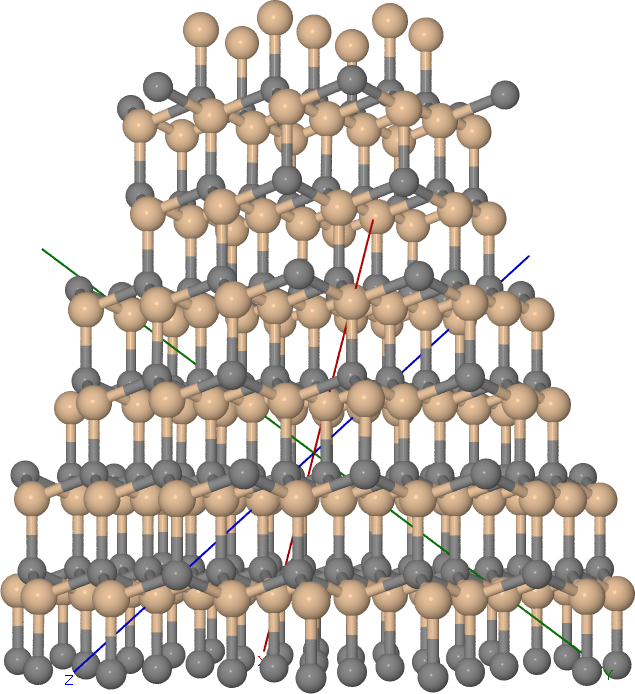
\includegraphics[width=0.6\textwidth]{srcexamples/cylinder.png}